\chapter{Experimental Setup}
\label{part_1}
This chapter is dedicated to setting up our environment for the research project. We need to select and get used to the tools required to perform the experiments. We also need to define methods to ensure reproducibility and legitimate comparison to state-of-the-art results. First, we introduce the tools and methods used throughout the study. After that, we experiment with \acrshort{lic} models and attempt to reproduce state-of-the-art results.

\section{Tools}
% As explained in Chapter \ref{sota}, current \acrshort{lic} models achieve impressive results: they provide encoding of images that contain very few bits while preserving their content. However, these models require a lot of processing power making them unsuitable for real-time application on resource constrained devices.
The goal of this project is to explore solutions to reduce the processing power used by current \acrshort{lic} models. In order to do that, it is necessary to have access to state-of-the-art \acrshort{lic} models, the image datasets used to train them and enough processing power to train and test such models.

CompressAI \cite{compressai} is a Python library for learned compression. Based on the well known machine learning library PyTorch, compressAI provides custom operations, layers and models for deep learning-based data compression and pre-trained end-to-end compression models for \acrshort{lic}. Amongs the pre-trained models is the model from Ballé et al. \cite{ballé2018variationalimagecompressionscale} that will be used throughout the project.

Usually, researchers train their models on the OpenImages dataset \cite{openimages} but pre-trained models on compressAI have been trained on the Vimeo90K dataset \cite{xue2019video}. In order to perform proper model comparisons, we will also use the Vimeo dataset for training during this project. For testing, two datasets will be used: the Kodak dataset \cite{kodak} and the dataset from the \acrfull{clic} \cite{clic}. Similarly to compressAI, visual inspection are also performed on a photograph of the port of Saint-Malo available in the GitHub repository of the library.

The computing power required for training and using models is offered by the GPU cluster of Télécom Paris.

\section{Method}
As for all research work, we need to define and share our methods for consistency throughout the study as well as reproducibility purpose. The following parts explain our choice of \acrshort{nn} as well as our training and testing methods.

\subsection{Neural Network}
For this project, we selected the scale hyperprior model introduced in 2018 by Ballé et al. \cite{ballé2018variationalimagecompressionscale}. This model has the advantage of being straightforward and yet complex enough to be challenging but not impossible to run on resource constrained computers. Its simple two stages architecture, schematised in Figure \ref{scale_hyperprior_1:a}, makes it a suitable candidate to perform \acrshort{kd} experiments using the latent spaces.

\begin{figure}[H]
    \centering
    \subfloat[Diagram showing the operational structure of the scale hyperprior compression model. Arrows indicate the flow of data, and boxes represent transformations of the data. Boxes labeled U | Q indicate either addition of uniform noise applied during training (producing vectors labeled with a tilde), or quantization and arithmetic coding/decoding during testing (producing vectors labeled with a hat).]{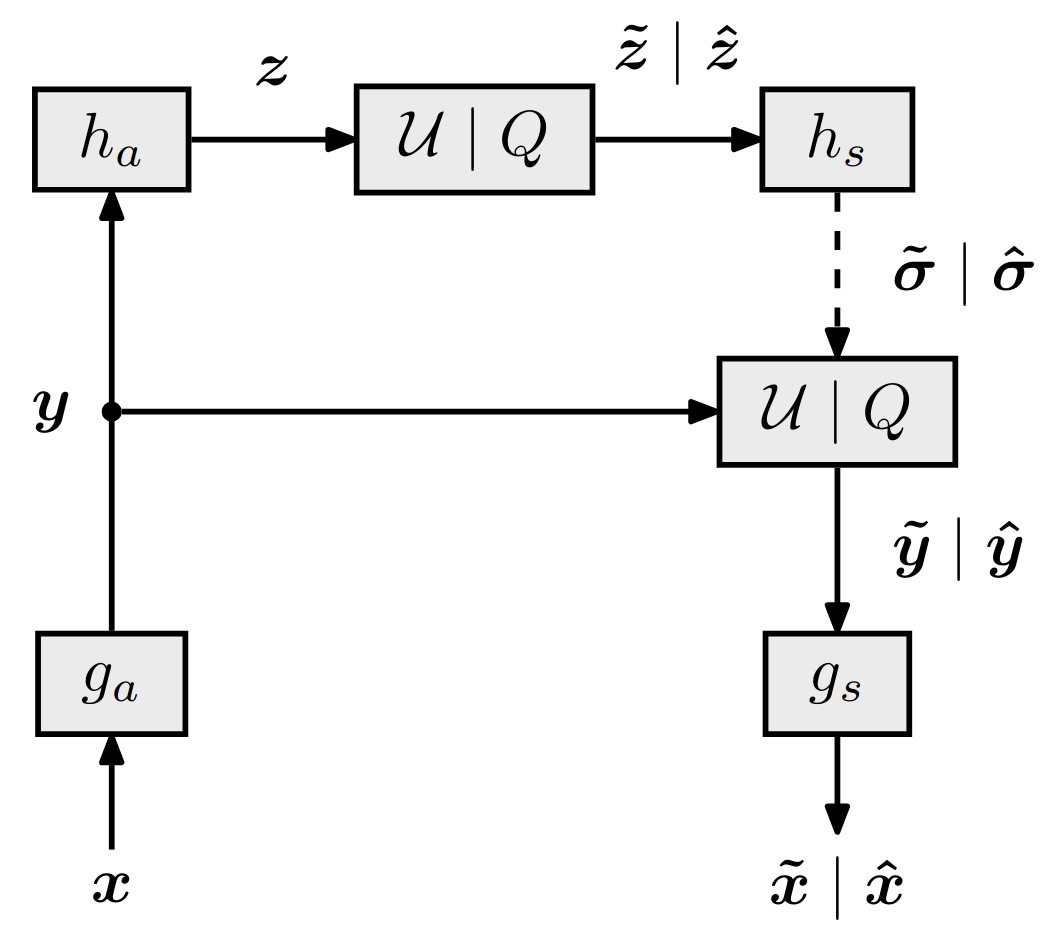
\includegraphics[width=6cm]{../img/scale_hyperprior_1.png} \label{scale_hyperprior_1:a}}
    \qquad
    \subfloat[Detailed architecture of the scale hyperprior compression model. The parameters N in the convolution layers designate the number of channels.]{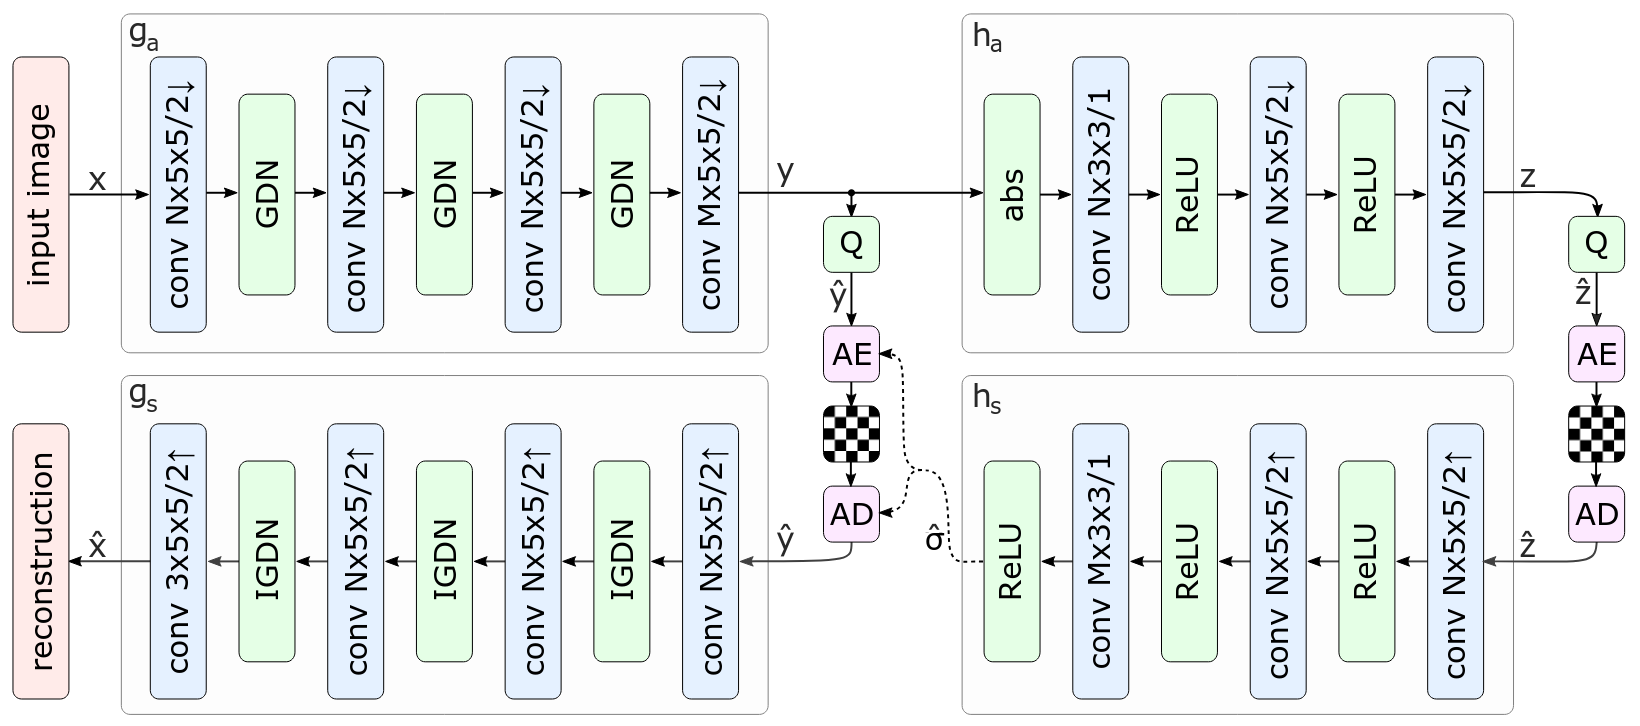
\includegraphics[width=10cm]{../img/scale_hyperprior_2.png} \label{scale_hyperprior_1:b}}
    \caption[Representations of the scale hyperprior model.]{Representations of the scale hyperprior model.}
    \label{kd_lic_2}
\end{figure}

% \begin{figure}
%     \centering
%     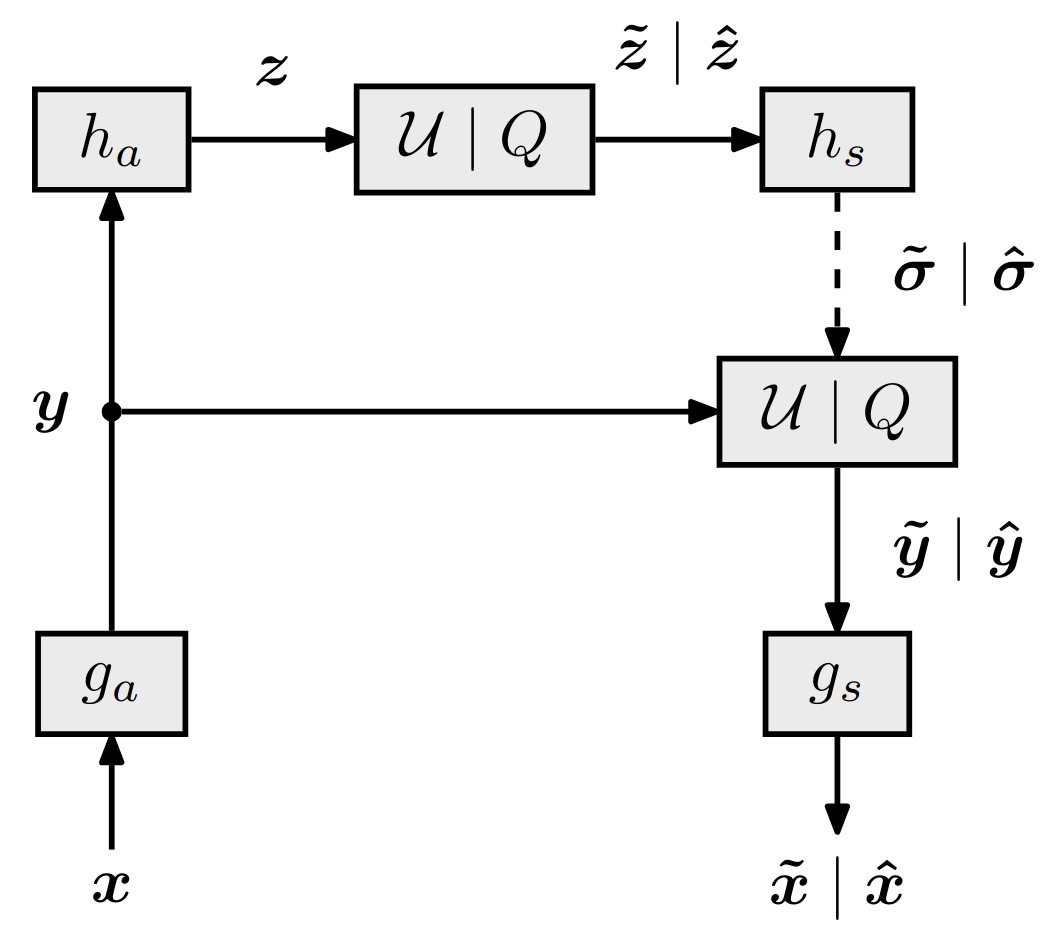
\includegraphics[width=8cm]{../img/scale_hyperprior_1.png}
%     \caption[Diagram showing the operational structure of the scale hyperprior compression model.]{Diagram showing the operational structure of the scale hyperprior compression model. Arrows indicate the flow of data, and boxes represent transformations of the data. Boxes labeled U | Q represent either addition of uniform noise applied during training (producing vectors labeled with a tilde), or quantization and arithmetic coding/decoding during testing (producing vectors labeled with a hat).}
%     \label{scale_hyperprior_1}
% \end{figure}

\subsection{Training Method}
\label{training_method}
As experiments parameters are not disclosed in the paper, we use compressAI pre-trained models as our baseline comparison. For fair comparison, we match as best as we can the training method described in the compressAI documentation \cite{compressai_train}. Models were trained between 4 and 5 million steps on 256x256 image patches randomly extracted and cropped from the Vimeo90K dataset. The batch size is 16 or 32 (we choose 16). The initial learning rate is 1e-4 and decreases over time (it is divided by 2 when the evaluation loss reaches a plateau). Two different metrics can be used: MSE or MS-SSIM. We keep the default metric (i.e. MSE) which corresponds to using the following loss function: \(L = \lambda\, 255^{2}\, D + R\) with \(D\) and \(R\) respectively the mean distortion and the mean estimated bit rate. The parameter \(\lambda\) allows to adjust the tradeoff between compression and image quality. Higher values give more importance to distortion encouraging the model to produce reconstructed images with high quality at the expense of bit rate. Inversely, lower values of \(\lambda\) imply more compression and more data loss. CompressAI proposes eight pre-trained models with different values of \(\lambda\) denoted by the argument \textsf{quality}. The correspondance between this argument and the value of \(\lambda\) is summarised in Table \ref{tab_quality_lambda}. It is important to note that the \textsf{quality} argument in compressAI also impacts the network architecture (number of channels and size of the latent space). Pre-trained models with \textsf{quality} lower or equal to 5 have 128 channels and a latent space with 192 dimensions. Other pre-trained models have 192 channels and a larger latent space with 320 components. 

\begin{table}[]
    \centering
    \begin{tabular}{|l|c|c|c|c|c|c|c|c|}
    \hline
    \textsf{quality}             & 1 & 2 & 3 & 4 & 5 & 6 & 7 & 8 \\ \hline
    Value of \(\lambda\) for MSE & 0.0018 & 0.0035 & 0.0067 & 0.0130 & 0.0250 & 0.0483 & 0.0932 & 0.1800 \\ \hline
    \end{tabular}
    \caption{Correspondance between the argument \textsf{quality} in compressAI and the value of \(\lambda\) when using MSE.}
    \label{tab_quality_lambda}
\end{table}

\subsection{Testing Method}
In order to compare our results to traditional codecs or other \acrshort{lic} \acrshort{nn}, different methods can be used. In this section, we present our qualitative and quantitative testing methods.

Visual inspection is the first method that comes to mind. When dealing with lossy compression, it is necessary to assess the visual fidelity of the compressed image compared to the original image. It is often useful to compare the outputs of different compression algorithms to compare them. In both cases, this is done by performing meticulous visual inspection on the entire image for overall evaluation or zoomed regions of interest to analyse details.

Visual inspection is subjective and should always be crossed with quantitative measures. Several metrics can be used. Based on what is used in the litterature, we opted for the following metrics.

Image compression deals with two caracteristics: image quality and bit rate. In our study, image quality is measured with \acrfull{psnr} (and \acrfull{msssim}) and bit rate in \acrfull{bpp}. Together, they define the \acrshort{rd} performance of a compression method.

\acrshort{rd} curves are a common tool to compare compression codecs and \acrshort{nn} architectures in \acrshort{lic}. It consists in plotting the average distortion in function of the average bit rate evaluated on a set of images. Using a range of \acrshort{rd} tradeoffs allows to easily evaluate and compare the overall \acrshort{rd} performance of an architecture.

These curves can then be used to compute the Bjøntegaard Deltas for both bit rate and image quality, respectively called BD-Rate and BD-\acrshort{psnr}. As explained in \cite{barman2024bjontegaarddeltabdtutorial}, these values characterise bit rate and quality differences between two \acrshort{rd} curves (using \acrshort{psnr} as distortion metric) by measuring the area between the curves. % TODO: more details

\section{State-of-the-art Results Reproduction}
Reproducing state-of-the-art results is key as it guarantees that our work environnement and methods are correct. This also provides shared baseline results between papers and our work that can be used to compare our future results. This task is divided in two parts. First, we try to train a single model and compare it to other pre-trained models. Then we train several models in order to produce \acrshort{rd} curves.

\subsection{Training a Model}
Using the training script provided by compressAI and following the method from Section \ref{training_method}, we train a scale hyperprior model with the compressAI argument \textsf{quality} set to 3, which corresponds to an architecture with 128 channels and 192 channels in the expansion layers (i.e. size of the latent space). The model is trained for approximately one million steps. After training, the model is evaluated and compared to conventional codecs as well as pre-trained models.

First, we try a single inference with this newly trained model. Figure \ref{balle_repro_1} shows that the reconstructed image (middle) is visually close to the original image. However, the difference between the two images (right) reveals that there are a lot of differences. These differences are located in the part of the image that contains details. These parts are often refered as containing high frequencies and are particularly hard to compress as opposed to low frequency areas that do not contain a lot of information (e.g. the plain blue sky in this picture). In this specific example, we found these differences are mainly noticeable in the clouds and the water that appear smoother on the reconstruction. Overall, the reconstruction is slightly blurrier than the original but the results are impressive given that this model is geared toward compression.

\begin{figure}
    \centering
    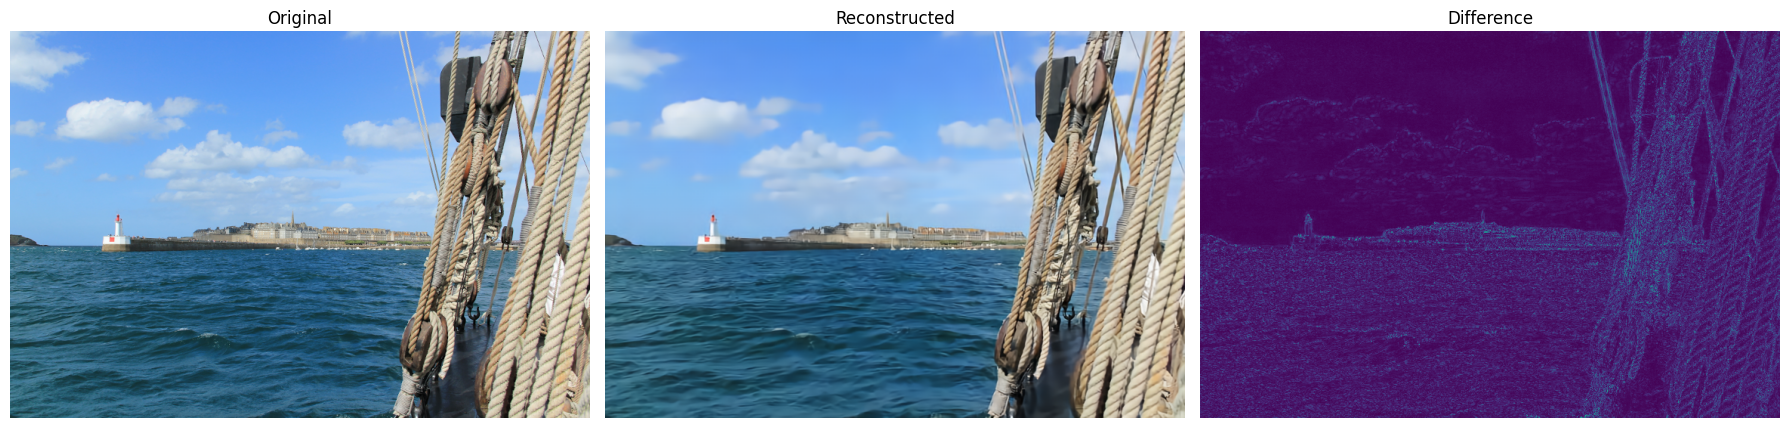
\includegraphics[width=15cm]{../img/balle_repro_diff.png}
    \caption[Comparison of the reconstructed image with the original image.]{Comparison of the reconstructed image with the original image. At first glance, the reconstructed image (middle) looks very similar to the original (left). Further inspection using the difference between the two images (right) unveils the loss of details attributed to lossy image compression/decompression. As expected, parts of the image containing details are the most affected whereas plain areas are mostly untouched.}
    \label{balle_repro_1}
\end{figure}

We proceed to compare our model to traditional methods. In the following paragraphs, we used JPEG and Webp to math the performance of our \acrshort{nn}-based solution. Figure \ref{balle_repro_2} shows encoding of the image at the same bit rate using different methods. It is clear that the \acrshort{nn} (top right) is the more accurate among the three methods used: JPEG introduces a lot of bloc artifacts and Webp does not retains as much details as the network, especially on the city buildings. This visual analysis is coherent with values of \acrshort{psnr}.

\begin{figure}
    \centering
    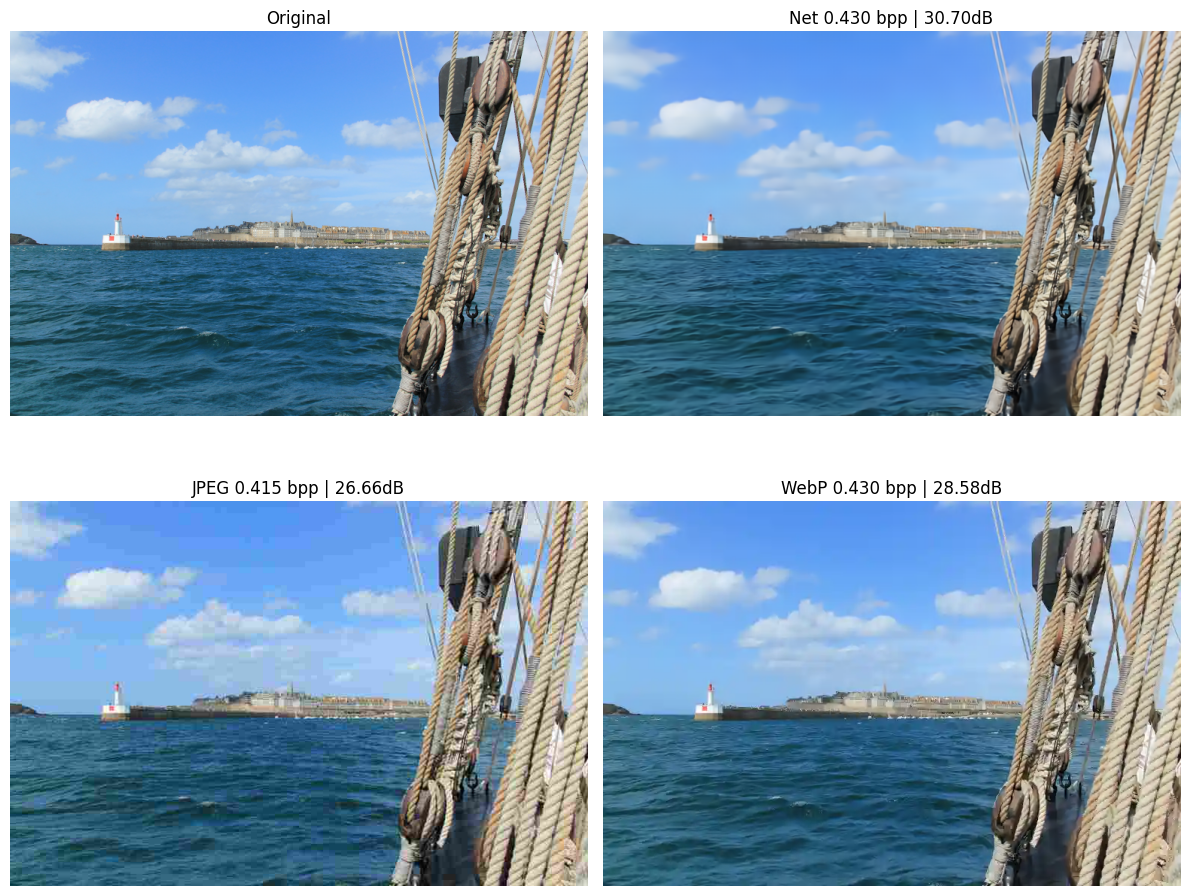
\includegraphics[width=15cm]{../img/balle_repro_bpp.png}
    \caption[Comparison to classical codecs (quality comparison at similar bit rate).]{Comparison to classical codecs (quality comparison at similar bit rate). Both qualitative and quantitative analysis show that the \acrshort{nn}-based approach is better than JPEG and Webp at a given bit rate.}
    \label{balle_repro_2}
\end{figure}

For the same distortion rate, our model has the smallest bit rate out of the three methods, that is to say: for the same visual quality, measured by the \acrshort{psnr}, the image is more compressed. Figure \ref{balle_repro_3} shows that it achieves less than 0.5 \acrshort{bpp} whereas traditional compression methods like Webp or JPEG achieve respectively 0.698 and 1.054 \acrshort{bpp}. We observe similar results when comparing methods at the same \acrshort{msssim}.

\begin{figure}
    \centering
    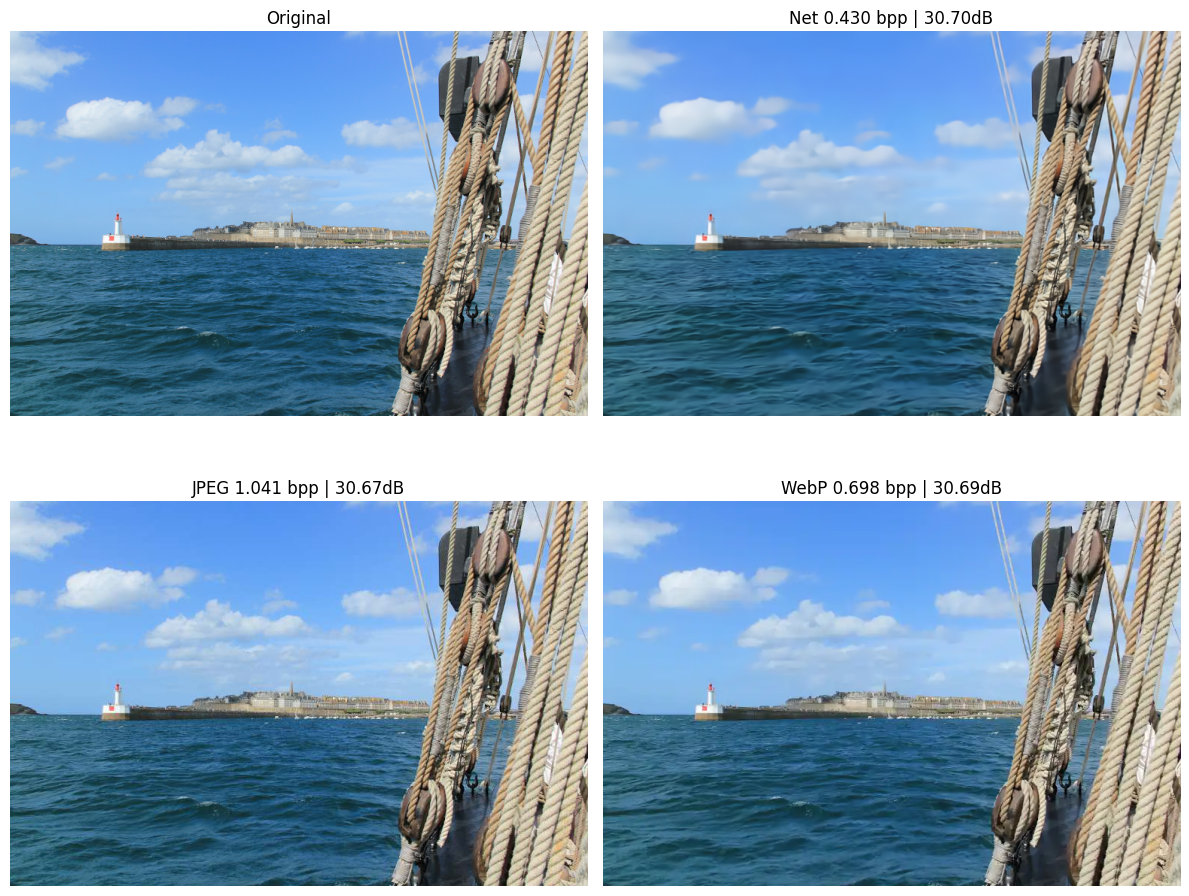
\includegraphics[width=15cm]{../img/balle_repro_psnr.png}
    \caption[Comparison to classical codecs (bit rate coparison at similar PSNR).]{Comparison to classical codecs (bit rate coparison at similar PSNR). This experiment highlights the clear advantage of \acrshort{lic} when models are trained to prioritise rate. For the same image quality (\acrshort{psnr}), JPEG and Webp results require more \acrshort{bpp}.}
    \label{balle_repro_3}
\end{figure}

It should however be noted that this particular model was trained to prioritise compression over image quality to a certain extent. Other models with different architectures and values of the parameter \(\lambda\) will perform differently. Litterature on the subject have prooved that \acrshort{lic} methods always outperform these codecs in \acrshort{rd} performance \cite{ballé2018variationalimagecompressionscale}.

Finally, we compare our model to other \acrshort{lic} models accessbible in the compressAI model zoo. Figure \ref{balle_repro_4} presents outputs from our model and various pre-trained models. Results are visually close but, closer inspection reveals that our model retains more details than the other pre-trained models. The differences are minimal but still visible in the ropes for instance. This is coherent with Figure \ref{balle_repro_5} that shows that our model, on this particular image sample, does not manage to reach bit rate performance as good as the other models but present better image quality instead. Other models perform worse in term of image quality but achieve a lower compression rate.

\begin{figure}
    \centering
    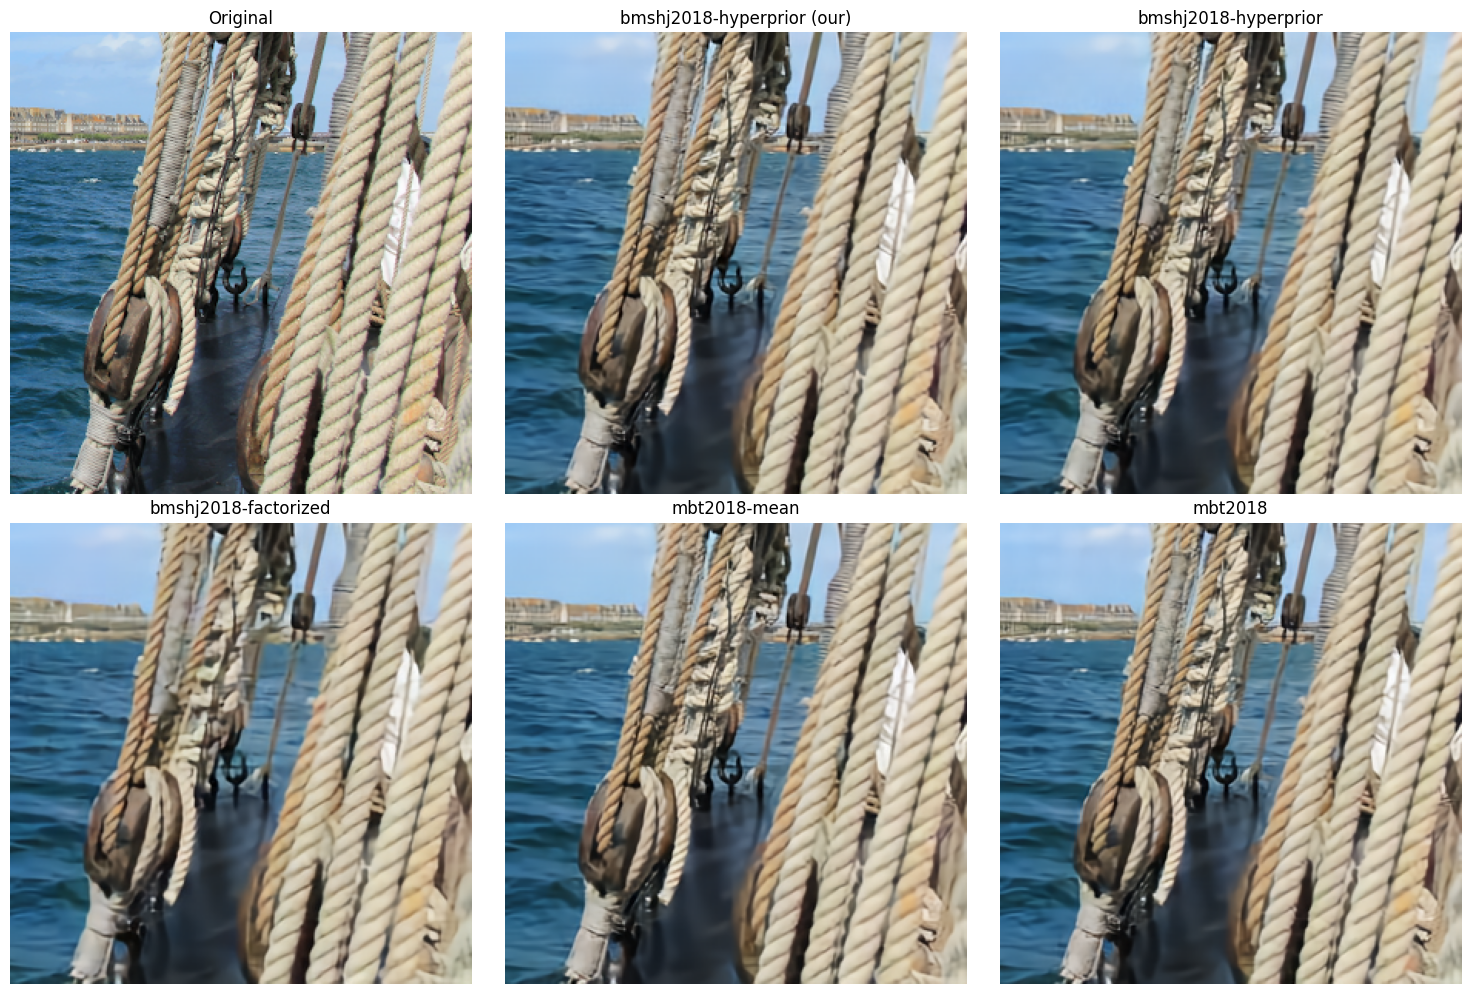
\includegraphics[width=15cm]{../img/balle_repro_models.png}
    \caption[Comparison to other \acrshort{lic} models (image reconstruction).]{Comparison to other \acrshort{lic} models (image reconstruction). Our model retains more details from the original image than the other pre-trained models.}
    \label{balle_repro_4}
\end{figure}

\begin{figure}
    \centering
    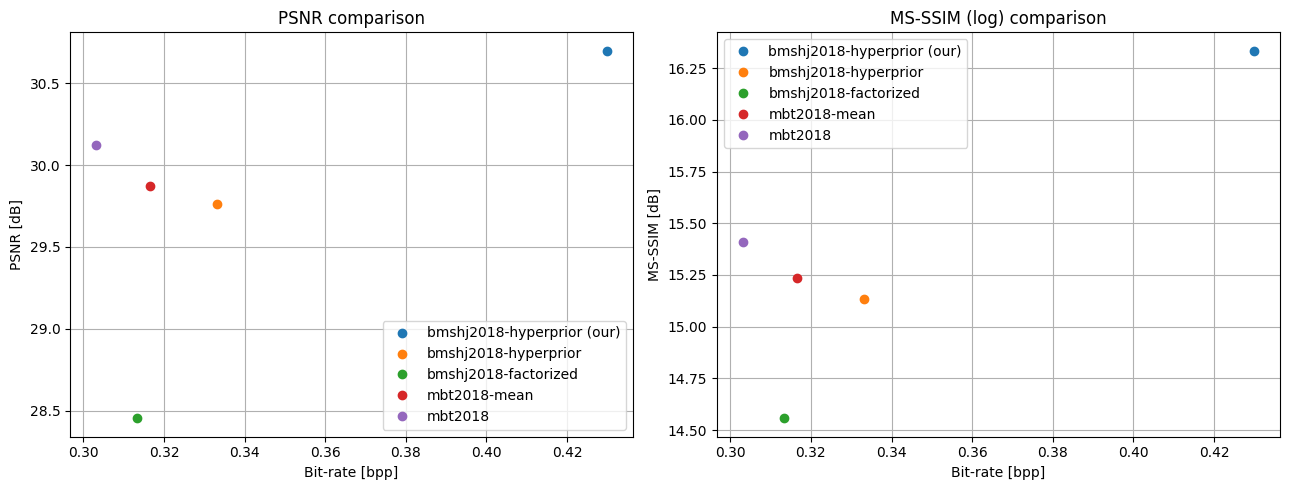
\includegraphics[width=15cm]{../img/balle_repro_rd_1.png}
    \caption[Comparison to other \acrshort{lic} models (\acrshort{rd}).]{Comparison to other \acrshort{lic} models (\acrshort{rd}). Our version of the scale hyperprior model outperforms all other models in terms of image quality. However, when it comes to \acrshort{bpp}, it delivers poor performance on this specific image.}
    \label{balle_repro_5}
\end{figure}

As evaluation on a single image is not representative, we also evaluate our scale hyperprior model on the entire Kodak dataset. We compare our model to compressAI pre-trained scale hyperprior models associated to the eight different values for the parameter \textsf{quality}. Models with \textsf{quality} value from 1 to 8 appear from left to right on the graph shown in Figure \ref{balle_repro_6} as lower quality implies lower bit rate. Our model was trained similarly as the model with \textsf{quality} 3 but the two models have different \acrshort{rd} performances. Our model favours a bit more image quality making it closer to the fourth pre-trained model. This small difference can be attributed to small difference in the training method (for instance, the batch sized used by compressAI was not properly disclosed) or simply run-to-run variance. As our model sits on the \acrshort{rd} curve of the pre-trained models, we can consider that it achieves state-of-the-art \acrshort{rd} performance. 

\begin{figure}
    \centering
    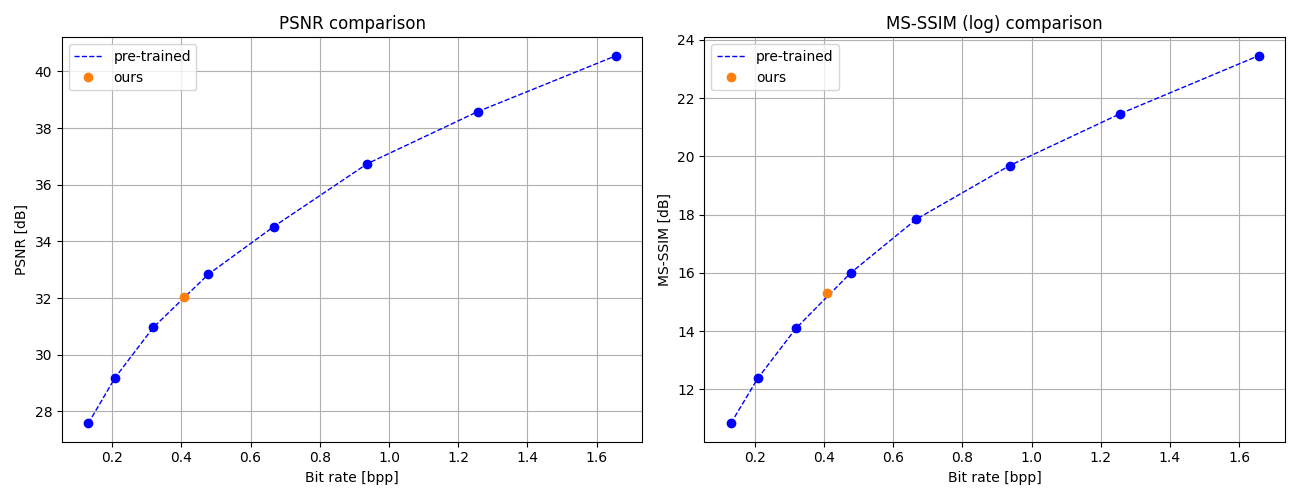
\includegraphics[width=15cm]{../img/balle_repro_rd_2.png}
    \caption[Comparison to pre-trained scale hyperprior models (\acrshort{rd}).]{Comparison to pre-trained scale hyperprior models (\acrshort{rd}). When properly compared to compressAI similar pre-trained models, our model reaches state-of-the-art \acrshort{rd} performance.}
    \label{balle_repro_6}
\end{figure}

This section shows that we are able to train a \acrshort{lic} \acrshort{nn} able to compress and decompress images while mostly preserving their content. Our model performs better than deterministic codecs like JPEG or Webp and produces results that are on par with other pre-trained \acrshort{nn}. Next section focuses on the model hyperparameters and the impact on the rate/distortion tradeoff.

\subsection{Rate-Distortion Tradeoff}
Different applications require different compromises in terms of bit rate and image quality. While bandwith limited video calls require low bit rate at the expense of image quality, transferring a single high resolution picture is more focused on image quality than limiting bandwidth use. Traditional codecs have settings to target bit rates values and \acrshort{lic} models can be trained with different \acrshort{rd} objectives in mind. In this section, we explore the range of \acrshort{rd} tradeoffs that can be achieved with \acrshort{lic} models.

Following the method presented in Section \ref{training_method}, we train eight different models: one for each value of the compressAI \textsf{quality} argument. That is to say, one for each couple of value of \(\lambda\) and corresponding model architecture. However, to quickly achieve comparable results, we limit the number of epochs to 65, just under what the GPU cluster is able to compute in 24 hours.

Let us start by passing a single image through the networks. The image from the Kodak datset is compressed and decompressed before being cropped for easier comparison. Figure \ref{bdpsnr_1} shows image reconstruction results from our models and pre-trained models for each settings. Models with the same \acrshort{rd} tradeoff from the compressAI zoo or trained from scratch produce results that are visually very similar. As expected, there is a discernable shift in image quality accross the range of models. Images related to lower values of \(\lambda\) (low bit rate and low quality) lack details and appear blurry. At the other end of the spectrum, images correponding to higher values of \(\lambda\) (high bit rate and high quality) look more detailed, sharp and similar to the original image. Notice how the details in the faces and the water appear when the value of \(\lambda\) increases.

\begin{figure}[H]
    \centering
    \subfloat[Our networks]{{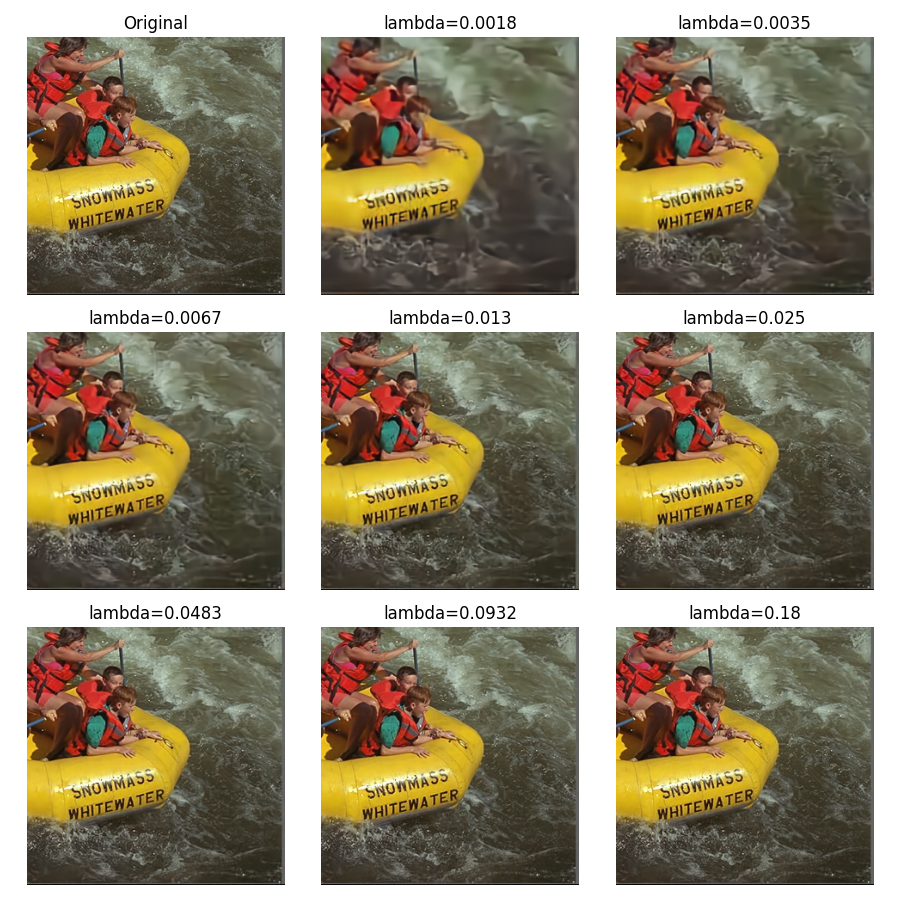
\includegraphics[width=8.5cm]{../img/bdpsnr_kodak_14.png} \label{bdpsnr_1:a}}}
    \subfloat[Pre-trained networks]{{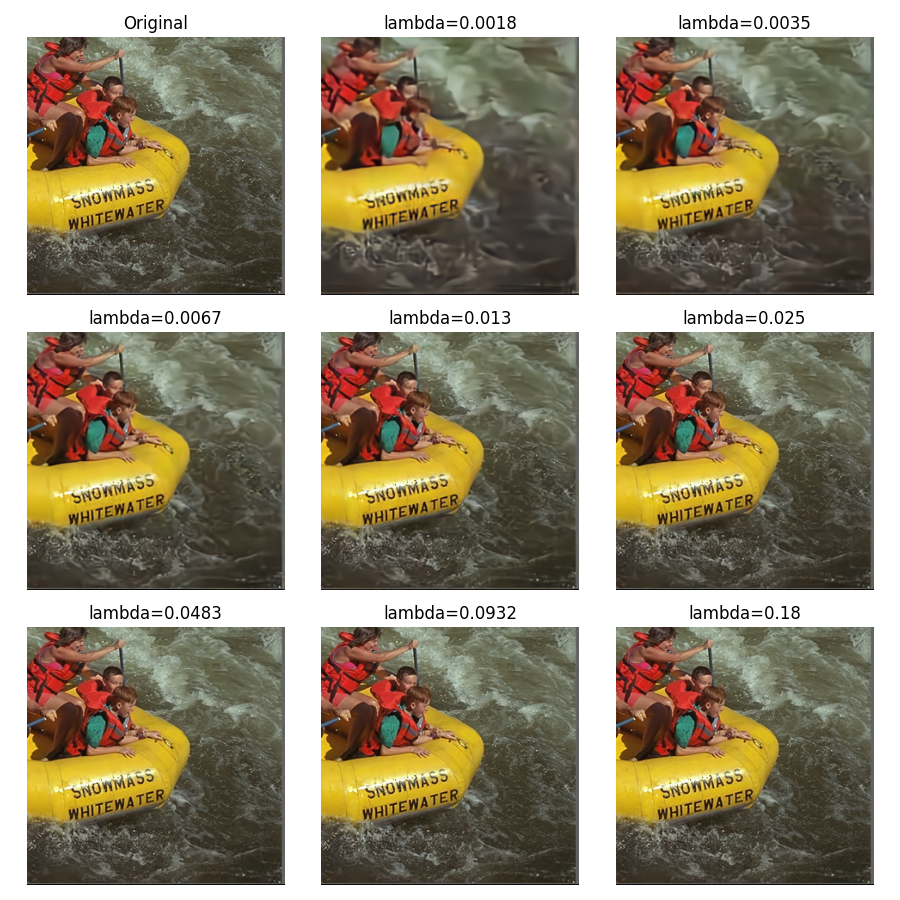
\includegraphics[width=8.5cm]{../img/bdpsnr_kodak_14_pretrained.png} \label{bdpsnr_1:b}}}
    \caption[Reconstruction results on image 14 of the Kodak dataset for different \acrshort{rd} tradeoffs.]{Reconstruction results on image 14 of the Kodak dataset for different \acrshort{rd} tradeoffs. For a given \acrshort{rd} compromise, our models produce results visually similar to the pre-trained models. The level of detail increases with the value of \(\lambda\), highlighting the \acrshort{rd} tradeoff.}
    \label{bdpsnr_1}
\end{figure}

We can produce \acrshort{rd} curve for this single image (Figure \ref{bdpsnr_2}). Consistently with our previous analysis, the curve shows that the visual fidelity increases as bit rates increase for both our models and pre-trained models. This also shows that for the same settings, models have close \acrshort{rd} performances. However, this quantitative assessment of the models reveals some differences. For lower bit rates our models performs on par with the pre-trained models but there is a slight difference for higher bit rates where our models do not reach the same level of image quality in terms of \acrshort{psnr}. This difference was difficult to measure visually.

\begin{figure}
    \centering
    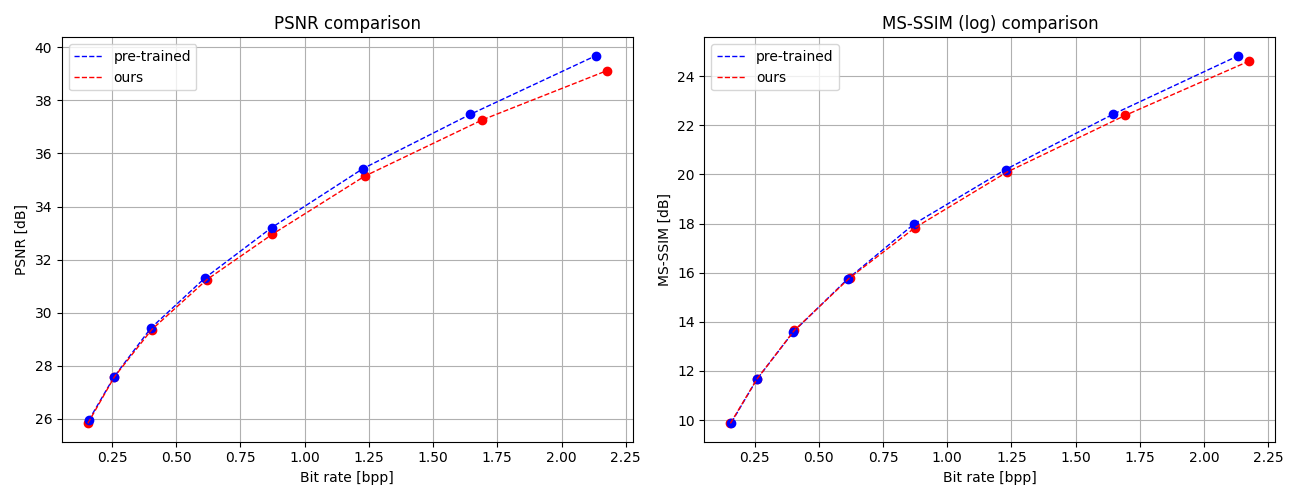
\includegraphics[width=15cm]{../img/bdpsnr_rd_kodak_14.png}
    \caption[Rate-distortion curve for image 14 of the Kodak dataset.]{Rate-distortion curve for image 14 of the Kodak dataset. Our low bit rate models manage to perform on par with the pre-trained models on this image instance. This is not the case for higher bit rates where our models do not manage to maintain the quality of the image.}
    \label{bdpsnr_2}
\end{figure}

It should be noted that the previous \acrshort{rd} curve corresponds to the results on a single image and thus is not representative of the overall performance of the models. By averaging metrics on the test dataset, we create an average \acrshort{rd} curve for the entire test dataset. This curve is shown in Figure \ref{bdpsnr_3}. Results are similar to those obtained in Figure \ref{bdpsnr_2}: on average, our models are very close to pre-trained models with a little disadvantage when dealing with higher bit rates. This translates in a BD-Rate of 4.38 \% and a BD-PSNR of -0.22 dB.

\begin{figure}
    \centering
    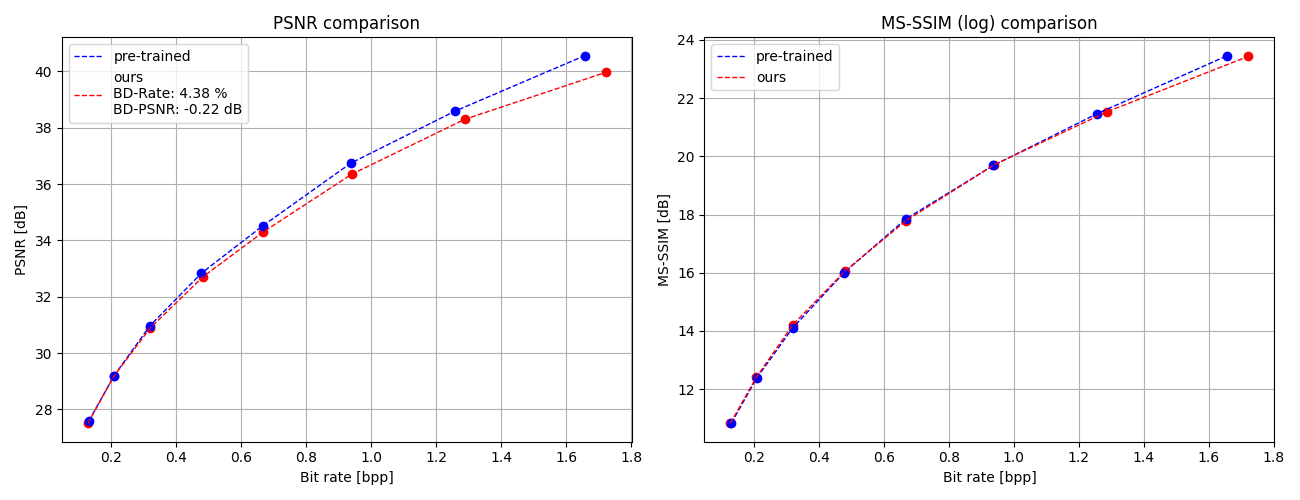
\includegraphics[width=15cm]{../img/bdpsnr_rd.png}
    \caption[Average \acrshort{rd} curve on the Kodak dataset.]{Average \acrshort{rd} curve on the Kodak dataset. Overall, our models are not as good as the pre-trained models. Ours present higher bit rate for a lower measured image quality, especially for high bit rates.}
    \label{bdpsnr_3}
\end{figure}

The selected model, more complex than a simple auto-encoder, makes use of side information obtained by an hyperprior. The results obtained by following the same method as compressAI show that we are able to achieve close to, if not state-of-the-art \acrshort{lic} results on traditional hardware using publicly available datasets and the processing power of the Télécom Paris GPU cluster. The performance of the models was assessed quantitatively using \acrshort{rd} performance and perceptually by visual inspection.